\documentclass{beamer}
\usepackage{graphicx}
\usetheme{Warsaw}
\usepackage[utf8]{inputenc}
\usepackage{tikz}
\usepackage{multirow}
\usepackage{multicol}
\setbeamercovered{transparent}% Dim out "inactive" elements
\usepackage[export]{adjustbox}

\usepackage[utf8]{inputenc}

\title{Assignment on Uncertainty}
\author{Ayesha Binte Mostofa \newline 1805062}
\institute
{
  Department of Computer Science and Engineering\\
  Bangladesh University of Engineering and Technology
}
\date{\today}
\begin{document}

\maketitle
\begin{frame}{Scenario}
\begin{center}
    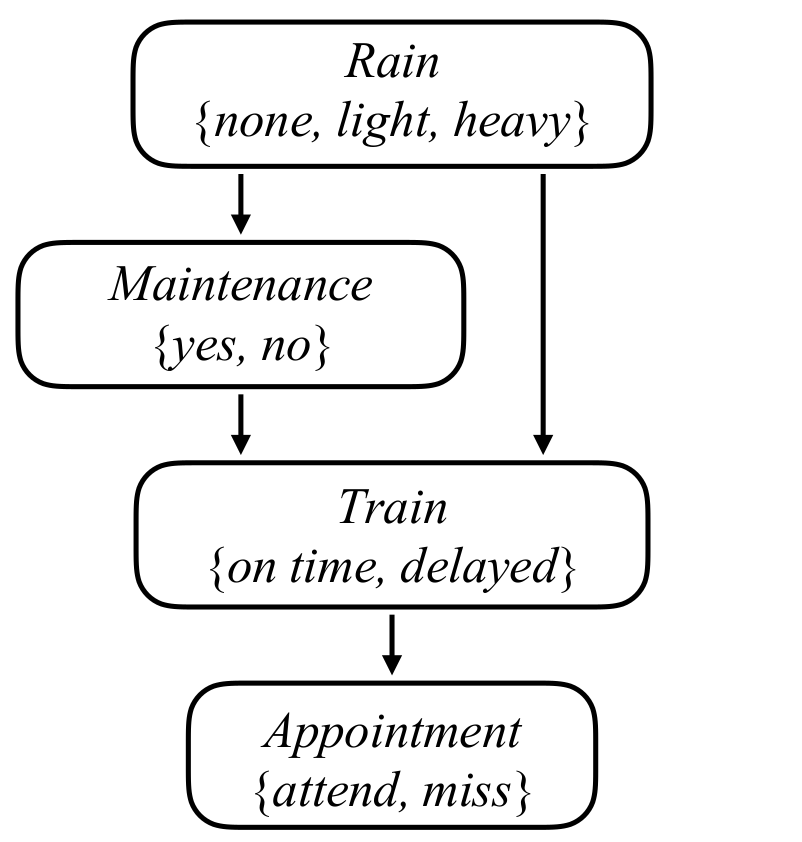
\includegraphics[scale=.25]{data.png}
\end{center}
\end{frame}
\begin{frame}{Given Problem}
\begin{itemize}
    \item  Given, Train state = delayed. Find updated probability distributions of other variables Rain and Maintenance. You must mathematically derive these probability distributions using the given formula.
\end{itemize}

\end{frame}
\begin{frame}{Distribution of Rain States}
\begin{center}
    \begin{tabular}{|c|c|c|}
         \hline
         \multicolumn{3}{|c|}{Rain States}\\
         \hline
         None & Light  & Heavy  \\
         \hline
         0.7 & 0.2  & 0.1  \\
         \hline
    \end{tabular}
\end{center}    
\end{frame}

\begin{frame}{Distribution of Maintenance States}
\begin{center}
    \begin{tabular}{|c|c|c|}
         \hline
         \multicolumn{3}{|c|}{Maintenance States}\\
         \hline
         Rain & Yes  & No  \\
         \hline
         None & 0.4  & 0.6  \\
         \hline
         Light & 0.2  & 0.8  \\
         \hline
         Heavy & 0.1  & 0.9  \\
         \hline
    \end{tabular}
\end{center}    
\end{frame}


\begin{frame}{Distribution of Train State -- Delayed}
\begin{center}
    \begin{tabular}{|c|c|c|}
         \hline
         \multicolumn{3}{|c|}{Train State : Delayed}\\
         \hline
         Rain & Maintenance & Delayed \\
         \hline
         None & Yes  & 0.2  \\
         \hline
         None & No  & 0.1 \\
         \hline
         Light & Yes  & 0.4  \\
         \hline
         Light & No  & 0.3  \\
         \hline
         Heavy & Yes  & 0.6  \\
         \hline
         Heavy & No  & 0.5  \\
         \hline
    \end{tabular}
\end{center}    
\end{frame}
\begin{frame}{Probability Calculation of Train States}
\begin{equation*}
    P(None,Yes,Delayed) = P(None)P(Yes|None)P(Delayed|None,Yes)
\end{equation*}
= 0.7*0.4*0.2 = 0.056
\newline
\begin{equation*}
    P(None,No,Delayed) = P(None)P(No|None)P(Delayed|None,No)
\end{equation*}
= 0.7*0.6*0.1 = 0.042
\newline
\end{frame}
\begin{frame}{Probability Calculation of Train States}
\begin{equation*}
    P(Light,Yes,Delayed) = P(Light)P(Yes|Light)P(Delayed|Light,Yes)
\end{equation*}
= 0.2*0.2*0.4 = 0.016
\newline
\begin{equation*}
    P(Light,No,Delayed) = P(Light)P(No|Light)P(Delayed|Light,No)
\end{equation*}
= 0.2*0.8*0.3 = 0.048
\newline
\end{frame}
\begin{frame}{Probability Calculation of Train States}
$P(Heavy,Yes,Delayed)=P(Heavy)P(Yes|Heavy)P(Delayed|Heavy,Yes)$ \newline
= 0.1*0.1*0.6 = 0.006
\newline\newline
    $P(Heavy,No,Delayed) = P(Heavy)P(No|Heavy)P(Delayed|Heavy,No)$\newline
= 0.1*0.9*0.5 = 0.045 
\newline
\end{frame}
\begin{frame}{Probability Distribution of Rain State}
    Marginalization of Rain States, given that train = delayed  \newline\newline
    {\small $P(None|delayed) = P(None, Yes|delayed) + P(None, No|delayed)$ \newline
        = .056 + .042 = .098
        \newline\newline
    $P(Light|delayed) = P(Light, Yes|delayed) + P(Light, No|delayed)$ \newline
        = .016 + .048 = .064 \newline\newline
        
    $P(Heavy|delayed) = P(Heavy, Yes|delayed) + P(Heavy, No|delayed)$ \newline
        = .006 + .045 = .051}
    \newline\newline
    Probability Distribution of Rain States : \newline
    P(Rain$|$train = delayed) \newline = $\alpha<$0.098,0.064,0.051$>$ \newline = $<$0.46,0.3005,0.2395$>$ 
    
\end{frame}

\begin{frame}{Probability Distribution of Maintenance State}
    Marginalization of Maintenance States, given that train = delayed \newline\newline
        {\small $P(Yes|delayed) = P(Yes,None|delayed) + P(Yes, Light|delayed) + P(Yes,Heavy|delayed)$ 
    = 0.056 + 0.016 + 0.006 = .078}\newline\newline
    {\small $P(No|delayed) = P(No,None|delayed) + P(No, Light|delayed) + P(No,Heavy|delayed)$
    = 0.042 + 0.048 + 0.045 = .135}
    \newline\newline
    Probability Distribution of Maintenance States : \newline 
    P(Maintenance$|$train = delayed) \newline = $\alpha<$.078,.135$>$ \newline = $<$0.3662,.6338$>$ 
\end{frame}

\begin{frame}{Code}
\begin{center}
    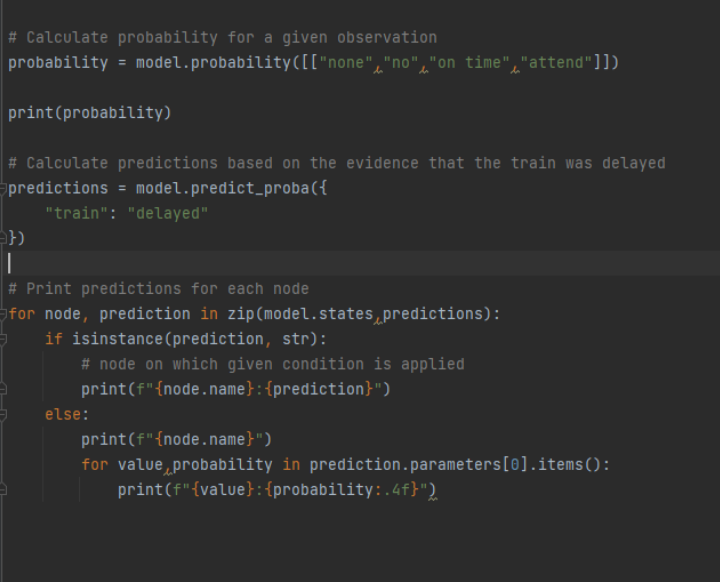
\includegraphics[scale=.5]{inference.png}
\end{center}
\end{frame}
\begin{frame}{Result}
\begin{center}
    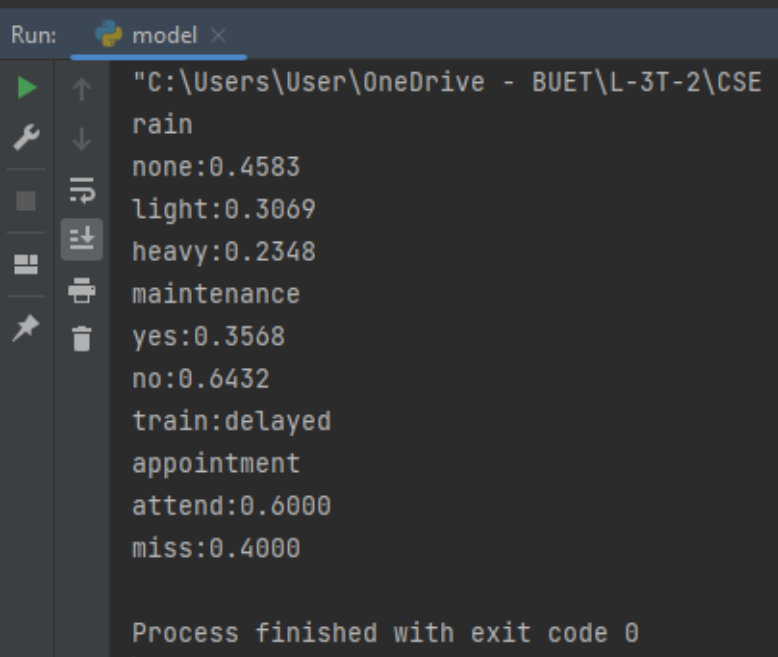
\includegraphics[scale=.5]{result.png}
\end{center}
\end{frame}


\end{document}
